\documentclass{beamer}

% \usepackage{beamerthemesplit} // Activate for custom appearance

\title{Matrix Approach to Linear Regresssion}
\author{Frank Wood}
%\date{\today}

\newcommand{\comment}[1]{}
\newcommand{\ponedec}{\mathcal{P}^\downarrow_1}
\newcommand{\pone}{\mathcal{P}_1}
\newcommand{\rank}[1]{\mathrm{RANK}\left[#1\right]}
\newcommand{\E}[1]{\mathrm{E}\left[#1\right]}
\newcommand{\py}{\mathcal{PY}}
\newcommand{\iid}{iid.}
\newcommand{\drawiid}{\stackrel{\text{iid}}{\sim}}
\newcommand{\vect}[1]{\mathbf{#1}}
\newcommand{\indicator}[1]{\text{I}\left[ #1 \right]}
\newcommand{\pdcoag}{PD(d_1,0)-\text{COAG}}
\newcommand{\todo}{\textbf{*TODO*}}
\newcommand{\igram}{\text{$\infty$-gram}}
\newcommand{\Prob}{\text{P}}

\def\mm{sequence memoizer }
\def\MM{SM }

\def\pibf{{\boldsymbol{\pi}}}
\def\kapbf{\boldsymbol{\kappa}}
\def\taubf{\boldsymbol{\tau}}
\def\thebf{\boldsymbol{\theta}}
\def\rhobf{\boldsymbol{\rho}}
\def\phibf{\boldsymbol{\phi}}
\def\pbf{\mathbf{p}}
\def\qbf{\mathbf{q}}
\def\bbf{\mathbf{b}}
\def\abf{\mathbf{a}}

\def\sbf{\mathbf{s}}
\def\tbf{\mathbf{t}}
\def\ybf{\mathbf{y}}
\def\bfA{\mathbf{A}}
\def\bfW{\mathbf{W}}
\def\bfy{\mathbf{y}}
\def\bfX{\mathbf{X}}
\def\wbf{\mathbf{w}}
\def\xbf{\mathbf{x}}
\def\rbf{\mathbf{r}}
\def\tbf{\mathbf{t}}
\def\kbf{\mathbf{k}}
\def\Xbf{\mathbf{X}}
\def\0bf{\mathbf{0}}
\def\Ibf{\mathbf{I}}
\def\phibf{\mathbf{\phi}}
\def\Phibf{\mathbf{\Phi}}
\def\disteq{{\stackrel{D}{=}}}
\def\EE{{\mathbb{E}}}

\def\phiv{\varphi}
\def\phivbf{\boldsymbol{\varphi}}

\def\Ocal{\mathcal{O}}

\DeclareMathOperator*{\Bet}{Beta} \DeclareMathOperator{\coag}{COAG}
\DeclareMathOperator{\frag}{FRAG} \DeclareMathOperator*{\rnk}{RANK}
\DeclareMathOperator*{\gem}{GEM} \DeclareMathOperator*{\pd}{PD}
\DeclareMathOperator*{\gd}{GDir} \DeclareMathOperator*{\Dir}{Dir}
\DeclareMathOperator*{\Ave}{\mathbb{E}}
\DeclareMathOperator*{\Var}{Var}

\begin{document}

\frame{\titlepage}

%\section[Outline]{}
%\frame{\tableofcontents}
%
%\section{Introduction}
%\subsection{Overview of Topics}
%
%\section{Bayesian Analysis}
%\subsection{Single Parameter Model}

\frame[t] {
 \frametitle{Random Vectors and Matrices}
 Let's say we have a vector consisting of three random variables\\
 \begin{center}
 \[\ybf= \begin{pmatrix}
 Y_1\\
 Y_2\\
 Y_3
 \end{pmatrix}\]
 \end{center}
 The expectation of a random vector is defined as\\
 \begin{center}
 \[\Ave(\bfy)=\begin{pmatrix}
 \Ave(Y_1)\\
 \Ave(Y_2)\\
 \Ave(Y_3)
 \end{pmatrix}\]
 \end{center}
}

\frame[t] {
 \frametitle{Expectation of a Random Matrix}
 The expectation of a random matrix is defined similarly
 \begin{center}
 $\Ave(\bfy)=[\Ave(Y_{ij})]~~~~~i=1,...n;j=1,...,p$
 \end{center}
}

\frame[t]  {
 \frametitle{Covariance Matrix of a Random Vector}
 The correlation of variances and covariances of and between the
 elements of a random vector can be collection into a matrix called
 the covariance matrix
 \begin{center}
 \[cov(\bfy) = \sigma^2\{\bfy\}=\begin{pmatrix}
 \sigma^2(Y_1) & \sigma(Y_1,Y_2) & \sigma(Y_1,Y_3)\\
 \sigma(Y_2,Y_1) & \sigma^2(Y_2) & \sigma(Y_2,Y_3)\\
 \sigma(Y_3,Y_1) & \sigma(Y_3,Y_2) & \sigma^2(Y_3)
 \end{pmatrix}\]
 \end{center}
 remember $\sigma(Y_2,Y_1)=\sigma(Y_1,Y_2)$
 so the covariance matrix is symmetric
}

\frame[t] {
 \frametitle{Derivation of Covariance Matrix}
 In vector terms the covariance matrix is defined by
 \begin{center}
 $\sigma^2\{\bfy\}=\Ave(\bfy-\Ave(\bfy))(\bfy-\Ave(\bfy))'$
 \end{center}
 because
 \begin{center}
 \[\sigma^2\{\bfy\}=\Ave(\begin{pmatrix}
 Y_1-\Ave(Y_1)\\
Y_2-\Ave(Y_2)\\
Y_3-\Ave(Y_3)\\
 \end{pmatrix} \begin{pmatrix}
 Y_1-\Ave(Y_1)&Y_2-\Ave(Y_2)&Y_3-\Ave(Y_3)
 \end{pmatrix}) \]
 \end{center}
}

\frame[t] {
 \frametitle{Regression Example}
 \begin{itemize}
 \item Take a regression example with $n=3$ with constant error
 terms $\sigma^2(\epsilon_i)$ and are uncorrelated so that
 $\sigma^2(\epsilon_i,\epsilon_j)=0$ for all $i \neq j$
 \item The covariance matrix for the random vector $\epsilon$ is
 \begin{center}
 \[ \bf \sigma^2(\mathbf{\epsilon})=\begin{pmatrix}
 \sigma^2 &0&0\\
 0&\sigma^2&0\\
 0&0&\sigma^2
 \end{pmatrix} \]
 \end{center}
 which can be written as $\bf \sigma^2\{\mathbf{\epsilon}\}=\sigma^2~\bf I$
 \end{itemize}
}

\frame[t] {
 \frametitle{Basic Results}
 If $\bf{A}$ is a constant matrix and $\bf{Y}$ is a random matrix then $\bf
 W=AY$\\
 is a random matrix
 \begin{center}
 $\Ave(\bfA)=\bfA$\\
 $\Ave(\bfW)=\Ave(\bfA\bfy)=\bfA\Ave(\bfy)$\\
 $\sigma^2\{\bfW\}=\sigma^2\{\bfA\bfy\}=\bfA\sigma^2\{\bfy\}\bfA'$
 \end{center}
}

\frame[t] {
 \frametitle{Multivariate Normal Density}
 \begin{itemize}
 \item Let $Y$ be a vector of $p$ observations
 \begin{center}
 \[\bf Y= \begin{pmatrix}
 Y_1\\
 Y_2\\
 .\\
 .\\
 .\\
 Y_p
 \end{pmatrix}\]
 \end{center}
 \item Let $\mu$ be a vector of $p$ means of each of the $p$
 observations
 \begin{center}
 \[\bf Y= \begin{pmatrix}
 \mu_1\\
 \mu_2\\
 .\\
 .\\
 .\\
 \mu_p
 \end{pmatrix}\]
 \end{center}
 \end{itemize}

}

\frame[t] {
 \frametitle{Multivariate Normal Density}
 let $\Sigma$ be the covariance matrix of Y
 \begin{center}
 \[\bf \Sigma= \begin{pmatrix}
 \sigma_1^2 & \sigma_{12} &...&\sigma_{1p}\\
 \sigma_{21} & \sigma_2^2 &... & \sigma_{2p}\\
 .\\
 .\\
 .\\
 \sigma_{p1}&\sigma_{p2}&...&\sigma_p^2
 \end{pmatrix}\]
 \end{center}
 Then the multivariate normal density is given by\\
 \[P(\mathbf{Y}|\mathbf{\mu},\mathbf{\Sigma})=\frac{1}{(2\pi)^{p/2}|\mathbf{\Sigma|}^{1/2}}exp(-\frac{1}{2}(\mathbf{Y}-\mathbf{\mu})'\mathbf{\Sigma}^{-1}(\mathbf{Y}-\mathbf{\mu}))\]
}

\frame[t] {
 \frametitle{Example 2d Multivariate Normal Distribution}
 \begin{figure}[h!]
   \centering
     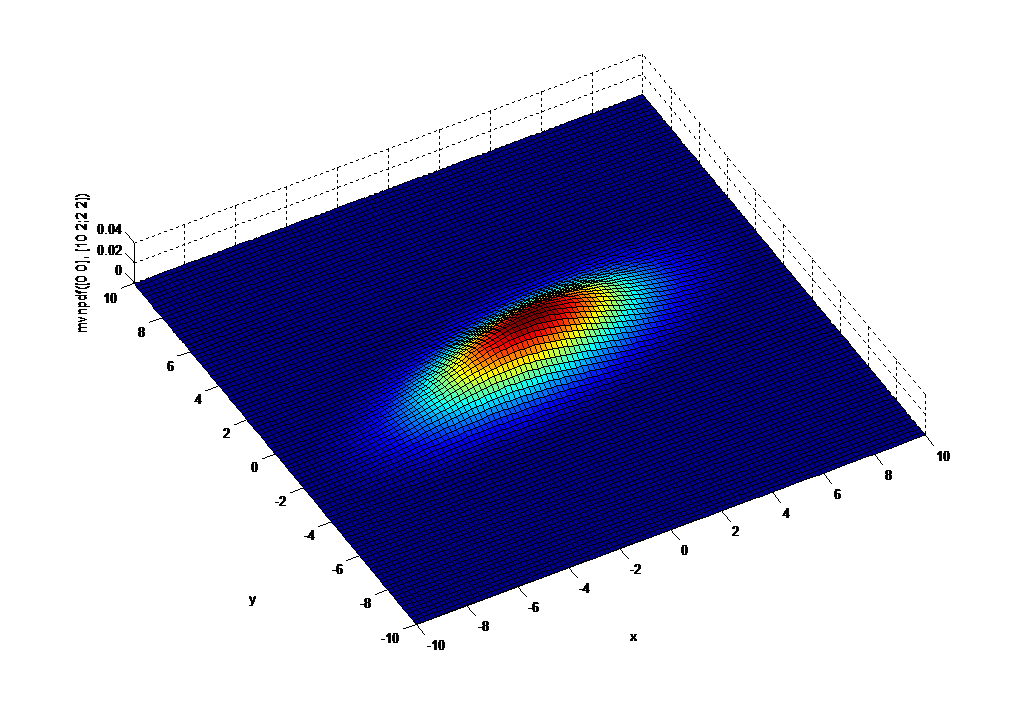
\includegraphics[scale=.4]{10.png}
 \end{figure}
}

\frame[t]{
 \frametitle{Matrix Simple Linear Regression}
 \begin{itemize}
 \item Nothing new-only matrix formalism for previous results
 \item Remember the normal error regression model
 \begin{center}
 $Y_i=\beta_0+\beta_1 X_i+\epsilon_i,~~\epsilon_i\sim N(0,\sigma^2),~~i=1,...,n$
 \end{center}
 \item Expanded out this looks like
 \begin{center}
 $Y_1=\beta_0+\beta_1 X_1+\epsilon_1$\\
 $Y_2=\beta_0+\beta_1 X_2+\epsilon_2$\\
 $...$\\
 $Y_n=\beta_0+\beta_1 X_n+\epsilon_n$\\
 \end{center}
\item which points towards an obvious matrix formulation.
 \end{itemize}
}

\frame[t] {
 \frametitle{Regression Matrices}
 \begin{itemize}
 \item If we identify the following matrices
 \begin{center}
 \[ \bf{Y} = \begin{pmatrix}
 Y_1\\
 Y_2\\
 .\\
 .\\
 .\\
 Y_n
 \end{pmatrix}~~\bf{X} =\begin{pmatrix}
 1&X_1\\
 1&X_2\\
 .\\
 .\\
 .\\
  1&X_n
 \end{pmatrix}~~\beta=\begin{pmatrix}
 \beta_0\\
 \beta_1\\
 \end{pmatrix} \epsilon=\begin{pmatrix}
 \epsilon_1\\
 \epsilon_2\\
 .\\
 .\\
 .\\
 \epsilon_n
 \end{pmatrix} \]
 \end{center}
 \item We can write the linear regression equations in a compact
 form $\bfy=\bfX \mathbf{\beta} + \bf \epsilon$
 \end{itemize}
}

\frame[t] {
 \frametitle{Regression Matrices}
 \begin{itemize}
 \item Of course, in the normal regression model the expected value
 of each of the $\epsilon$'s is zero, we can write $\Ave(\bfy)=\bfX \beta$
 \item This is because
 \begin{center}
 $\Ave(\epsilon)=\bf {0}$~~\[\begin{pmatrix}
 \Ave(\epsilon_1)\\
 \Ave(\epsilon_2)\\
 .\\
 .\\
 .\\
 \Ave(\epsilon_n)
 \end{pmatrix}=\begin{pmatrix}
 0\\
 0\\
 .\\
 .\\
 .\\
 0
 \end{pmatrix}\]
 \end{center}

 \end{itemize}

}

\frame[t] {
 \frametitle{Error Covariance}
 Because the error terms are independent and have constant variance
 $\sigma^2$
 \begin{center}
 \[\sigma^2\{\epsilon\}=\begin{pmatrix}
 \sigma^2&0&...&0\\
 0&\sigma^2&...&0\\
 ...\\
 0&0&...&\sigma^2
 \end{pmatrix}\]\\
 $\sigma^2\{\epsilon\}=\sigma^2\bf{I}$
 \end{center}
 }

\frame[t] {
 \frametitle{Matrix Normal Regression Model}
 In matrix terms the normal regression model can be written as
 \begin{center}
 $\bfy=\bfX\beta+\epsilon$
 \end{center}
 where $\Ave(\epsilon)=\bf{0}$ and $\sigma^2\{\epsilon\}=\sigma^2 \bf{I}$, i.e.~$\epsilon \sim N(\bf0,\sigma^2\Ibf)$

}

\frame[t] {
 \frametitle{Least Square Estimation}
 If we remember both the starting normal equations that we derived
 \begin{center}
 $nb_0+b_1\sum X_i=\sum Y_i$\\
 $b_0 \sum X_i+b_1 \sum X_i^2=\sum X_i Y_i$
 \end{center}
 and the fact that
 
 \[ \bf X'X= \begin{bmatrix}
1&1&...&1\\
 X_1 & X_1 &...&X_n
\end{bmatrix}
\begin{bmatrix}
1&X_1\\
1&X_2\\
.\\
.\\
.\\
1&X_n
\end{bmatrix}=\begin{bmatrix}
n&\sum X_i\\
\sum X_i & \sum X_i^2
\end{bmatrix} \]

\[ \bf X'y= \begin{bmatrix}
1&1&...&1\\
 X_1 & X_1 &...&X_n
\end{bmatrix}
\begin{bmatrix}
Y_1\\
Y_2\\
.\\
.\\
.\\
Y_n\\
\end{bmatrix}=\begin{bmatrix}
\sum Y_i\\
\sum X_i Y_i
\end{bmatrix} \]
 }
 
 \frame[t] {
 \frametitle{Least Square Estimation}
 Then we can see that these equations are equivalent to the following
 matrix operations
 \begin{center}
 $\bf X'X~b=X'y$
 \end{center}
 with
 \begin{center}
 \[\bf{b}=\begin{pmatrix}
 b_0\\
 b_1
 \end{pmatrix}\]
 \end{center}
 with the solution to this equation given by \[ \bbf=(\Xbf'\Xbf)^{-1}\Xbf'\ybf\]
 when $(\Xbf'\Xbf)^{-1}$ exists.
}

 \frame[t] {
 \frametitle{When does $(\Xbf'\Xbf)^{-1}$ exist?}
 $\Xbf$ is an $n\times p$ (or $p+1$ depending on how you define $p$) design matrix.  
\bigskip

$\Xbf$ must have full column rank in order for the inverse to exist, i.e. $rank(\Xbf) = p \implies (\Xbf'\Xbf)^{-1}$ exists.


}











\end{document}
